\chapter{Trave: momento flettente SLU}
\section{Progetto della sezione maggiormente sollecitata}
In riferimento ai valori mostrati in precedenza nella tabella \ref{tab:trave_ULS_momento} a pagina \pageref{tab:trave_ULS_momento}, si progetta ora la sezione in calcestruzzo armato considerando quella maggiormente sollecitata.
Nel caso in esame è quella in appoggio 5 avente un momento pari a $\SI{-247.45}{\kilo\newton\metre}$.
Essendo soggetta a momento flettente negativo, sarà considerata invertita rispetto la disposizione reale e considerata quindi a momento flettente positivo, con le armature invertite. 
A tale scopo verrà utilizzata la nomenclatura \emph{inv.} nelle tabelle a seguire per indicare tutte quelle sezioni che sono state invertite.

\begin{figure}[ht]
  \centering
  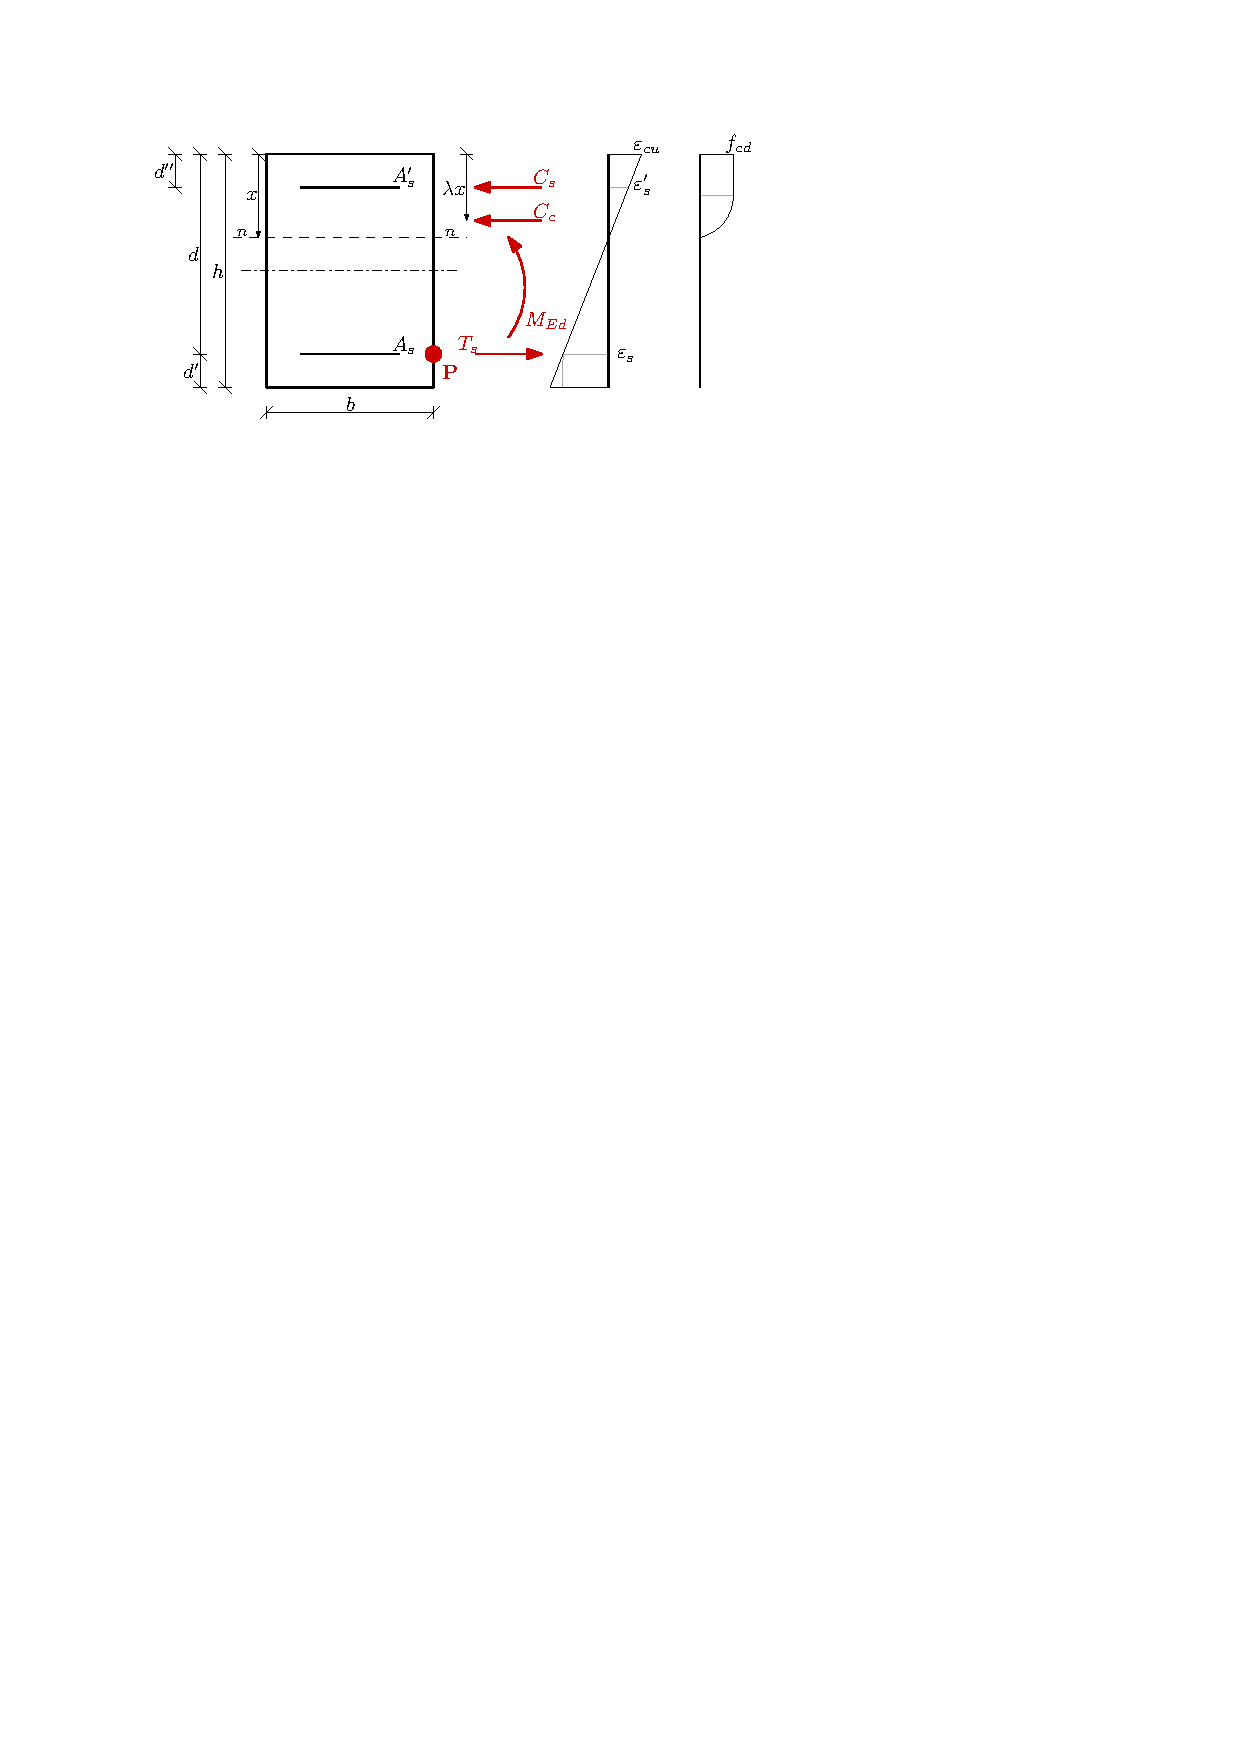
\includegraphics[height=0.25\textheight]{IMG/IPE_slu_progetto.pdf}
  \caption{Convenzione e nomenclatura utilizzata per il progetto agli SLU}
  \label{fig:slu_progetto}
\end{figure}

Utilizzando la convenzione di segni riportata in figura \ref{fig:slu_progetto} e il polo $\mathbf{P}$ riportato, è possibile scrivere il sistema per determinare i valori dell'altezza utile $d$ e della quantità di armature inferiori $A_s$ che soddisfano il momento flettente applicato. 
\begin{equation}
  \begin{cases}
    C_c + C_s - T_s = 0 \\
    C_c \left(d - \lambda\,x\right) + C_s \left(d - d^{\prime\prime}\right) = M_{Ed}
  \end{cases}
\end{equation}
Sistema che è possibile risolvere esplicitando i valori delle risultanti e facendo delle ipotesi per ridurre il numero di variabili. 
Si fissa il rapporto di armatura $\beta = 0.2$, ovvero pari al minimo possibile, in quanto il momente flettente a segno opposto nella sezione in esame è nullo.
Inoltre il progetto è vincolato, pertanto la base è imposta a \SI{300}{\milli\metre}.
Come copriferri $d^\prime,d^{\prime\prime}$ si scelgono entrambi uguali e pari a \SI{40}{\milli\metre}.
Infine si fissa il pieno utilizzo delle capacità meccaniche dei materiali: per cui l'acciaio superiore risulta snervato, e di conseguenza $\sigma_s^\prime = f_{yd}$, e il calcestruzzo a collasso, e di conseguenza $\sigma_c = f_{cd}$.
I coefficienti $\lambda$ e $\psi$ sono quelli del campo 3 e quindi pari a $\frac{17}{21}$ e $\frac{99}{238}$, mentre $\xi$ è pari a quella della retta limite tra campo 2 e 3, ovvero: $\xi_{2-3} = \frac{\varepsilon_{cu}}{\varepsilon_{cu} + \varepsilon_{su}} = \num{0.25926}$.

Il sistema espanso risulta:
\begin{equation}
  \begin{cases}
    b \, \psi \, \xi \, d \, f_{cd} + \beta \, A_s \, f_{yd} - A_s \, f_{yd} = 0 \\
    b \, \psi \, \xi \, d \, f_{cd} \left(d - \lambda\,x\right) + \beta \, A_s \, f_{yd} \left(d - d^{\prime\prime}\right) = M_{Ed}
  \end{cases}
\label{eq:sistemaSLU}
\end{equation}
e risolvendolo si ottengono i seguenti valori:
\begin{equation}
  \hookrightarrow \quad
  \begin{cases}
    A_s &= \SI{1416.82}{\milli\metre\squared} \\
    A_s^\prime &= \SI{283.36}{\milli\metre\squared} \\
    d &= \SI{497.23}{\milli\metre}
  \end{cases}
\end{equation}

Si vuole cercare di avere un'altezza totale $h = \SI{500}{\milli\metre}$, per cui si sceglie un'altezza utile $d = \SI{460}{\milli\metre}$ inferiore a quella ottenuta dal sistema. 
I valori di armature $A_s$ sono soddisfatti con ad esempio 8Ø16, 6Ø18 o 5Ø20, aventi rispettivamente \SI{1608}, \SI{1527}, \SI{1570}{\milli\metre\squared} di area.
Avendo problemi riguardo la base minima su cui si dispongono le barre, il diametro da 16 non può essere utilizzato. 
Vengono perciò adottati i 6Ø18 che rispettano i requisiti, come di seguito dimostrato:
\begin{equation}  
  \begin{split}
    b_{min} &= 2 \cdot \text{copriferro} + 2 \cdot \varnothing_\textup{staffe} + n_\textup{barre} \cdot \varnothing_\textup{barre} + \left( n_\textup{barre} - 1 \right) \cdot \text{dist}_\textup{barre}  \\
    &= 2 \cdot 20 + 2 \cdot 10 + 6 \cdot 18 + \left( 6 - 1 \right) \cdot 25 \quad \si{\milli\metre}\\
    &= \SI{293}{\milli\metre} < b = \SI{300}{\milli\metre} \quad \checked ,
  \end{split}
\end{equation}
mentre per le armature superiori si scelgono 2Ø18 con unica funzione di reggi staffa.

Un ulteriore controllo da fare è il rispetto del minimo e massimo di armatura rispetto la sezione di calcestruzzo.
Si utilizzano come aree di acciaio di verifica 6Ø18 e 2Ø18, che sono il massimo e minimo valore che si prevede debbano essere necessari lungo tutta la trave.
\begin{equation}
  A_s =
  \begin{bmatrix}
    \SI{1527}{\milli\metre\squared} \\
    \SI{509}{\milli\metre\squared}
  \end{bmatrix}
  \begin{cases}
    < 0.04 \, A_c = 0.04 \, b \, h = \SI{6000}{\milli\metre\squared} \\
    > 0.003 \, A_c = 0.003 \, b \, h = \SI{414}{\milli\metre\squared}
  \end{cases}
  \quad \checked
\end{equation}
inoltre si deve avere un quantitativo mimino specificatamente in zona tesa
\begin{equation}
  A_s =
  \begin{bmatrix}
    \SI{1527}{\milli\metre\squared} \\
    \SI{509}{\milli\metre\squared}
  \end{bmatrix}
  > \max\left(0.26 \, b_\textup{t} \, d \frac{f_{ctm}}{f_{yk}}; \, 0.0013 \, b_\textup{t} \, d\right) = \max\left(204.5; \, 179.4\right) = \SI{204.5}{\milli\metre\squared}
  \quad \checked
\end{equation}
\section{Verifica della sezione maggiormente sollecitata}
Per verificare se la sezione progettata è resistente al momento flettente appliccato, occorre innanzitutto controllare in quale campo deformativo essa appartiene e, successivamente, applicare l'equilibrio alla rotazione per trovare l'$M_{Rd}$ cercato.

Come prima cosa si verificano quali campi possono esistere, si ha infatti:
\begin{equation}
  d^{\prime\prime} = \SI{40}{\milli\metre} <  d^{\prime\prime}_{\xi_{2-3}} = \frac{\varepsilon_{cu} - \varepsilon_{se}^\prime}{\varepsilon_{cu} - \xi_{2-3}} =\SI{55.77}{\milli\metre} \quad \Longrightarrow  \quad \exists \; \text{Campo 2A, 2B, 3B}
\end{equation}

Si ipotizza essere in campo 3B, corrispondente ad armature inferiori e superiori plasticizzate.
Dall'equazione di equilibrio alla traslazione riportata precedentemente nelle \ref{eq:sistemaSLU} si ricava
\[
  \xi_{3B} = \frac{f_{yd} (A_s - A_s^\prime)}{f_{cd} \psi b h} = \num{0.25166} > \xi_{2-3} = \num{0.25926}
\]
pertanto l'ipotesi di campo 3B è errata e l'asse neutro è inferiore.

Si ipotizza essere in campo 2B, quindi con armature plasticizzate e con il tratto parabolico del legame costitutivo del calcestruzzo non pienamente sviluppato.
Ipotizzando il calcestruzzo non essere a collasso, ovvero: $\varepsilon_{c2} < \varepsilon_{c} , \varepsilon_{cu}$, i coefficienti $\psi$ e $\lambda$ valgono:
\[
  \begin{split}
    \psi_{2} &= 1 - \frac{1}{3}   \frac{\varepsilon_{c2}}{\varepsilon_{su}}\frac{1-\xi}{\xi}\\
    \lambda_{2} &= \frac{\left( 6\varepsilon_{su}^2 + 4\varepsilon_{su}\varepsilon_{c2} + \varepsilon_{c2}^2 \right)\xi^2 -2\varepsilon_{c2}^2 \xi + \varepsilon_{c2}^2 + 4\varepsilon_{su}\varepsilon_{c2}\xi}{4\varepsilon_{su}\xi \left[ \left( 3\varepsilon_{su} + \varepsilon_{c2} \right)\xi - \varepsilon_{c2} \right]}
  \end{split}  
\]
e risolvendo come prima rispetto $\xi$, si ottiene:
\begin{equation}
  \xi_{2B} = \num{0.25349}
\end{equation}
la quale soddisfa le ipotesi di altezza dell'asse neutro e delle condizioni di tensione ipotizzate:
\begin{equation}
  \begin{split}
    \varepsilon_{s}^\prime &= \varepsilon_{su}\,\frac{\xi_{2B} - \delta^{\prime\prime}}{1-\xi_{2B}} = \SI{2.231}{\permille} > \varepsilon_{se}^\prime = \SI{1.863}{\permille}\\
    \varepsilon_{c2} = \SI{2}{\permille} < \varepsilon_{c} &= \varepsilon_{su} \,\frac{\xi_{2B}}{1-\xi_{2B}} =  \SI{3.395}{\permille} < \varepsilon_{cu} = \SI{3.5}{\permille}\\
    \varepsilon_{s} &= \varepsilon_{su} = \SI{10}{\permille}
  \end{split}
  \quad \checked \quad .
\end{equation}

È ora possibile sostituire $\xi_{2B}$ nelle precedenti equazioni per ricavare i veri valori di $\psi$ e $\lambda$, ed ottenere infine, dalla seconda delle \ref{eq:sistemaSLU}, un momento resistente pari a:
\begin{equation}
  \begin{split}
    \psi_{2} &= \num{0.803671}\\
    \lambda_{2} &= \num{0.413826}\\
    M_{Rd} &= \SI{247.634}{\kilo\newton\metre} > M_{Ed} = \SI{247.450}{\kilo\newton\metre} \quad \checked \quad .
  \end{split}
\end{equation}
%--- LOG --- 
%Ipotesi di campo 3B, calcolo della retta limite 2-3
%xi_23 = 0.25926
%Esiste campo 2a, 2b, 3b perchè d2 = 40.00 < d2_xi23 = 55.77 mm
%xi_3 = 0.25166
%Ipotesi di campo 3 errata! xi_3 = 0.25166 < xi_23 = 0.25926 ma devo comunque verificare tramite es1 perché ho usato hp di es plasticizzato del 3B
%Essendo d2 = 40.00000 < d2_xi23 = 55.76720, non può esserci il campo 3A
%Calcolo xi con ipotesi di campo 2B: armature superiori snervate
%xi_2b = 0.25349
%!!!!!!!!!!!!!!verifica del ec da fare
%Ipotesi armature superiori snervate ok! es1 = 0.22308% > di ese1 = 0.18634%

%campo': '2B',
% 'ec': 0.0033956711163810735,
% 'es': 0.01,
% 'es1': 0.002230830149739241,
% 'xi': 0.2534901825283417,
% 'psi': 0.8036716031035525,
% 'lamb': 0.4138260346516767,
% 'Nrd': 0.0,
% 'Mrd': 247633547.16419485
\section{Progetto e verifica di tutte le altre sezioni}
Per eseguire in modo rapido il progetto di tutte le sezioni coinvolte all'interno della trave si è fatto uso del diagramma dell'azione del momento flettente sollecitante a cui sono stati sovrapposti i momenti resistenti di sezioni simili ma con quantitativi di barre diverse. 
Tale rappresentazione è visibile in figura \ref{fig:ULS_M_progettazioneTramiteMomentiResistenti}. 
\begin{figure}[htb]
  \centering
  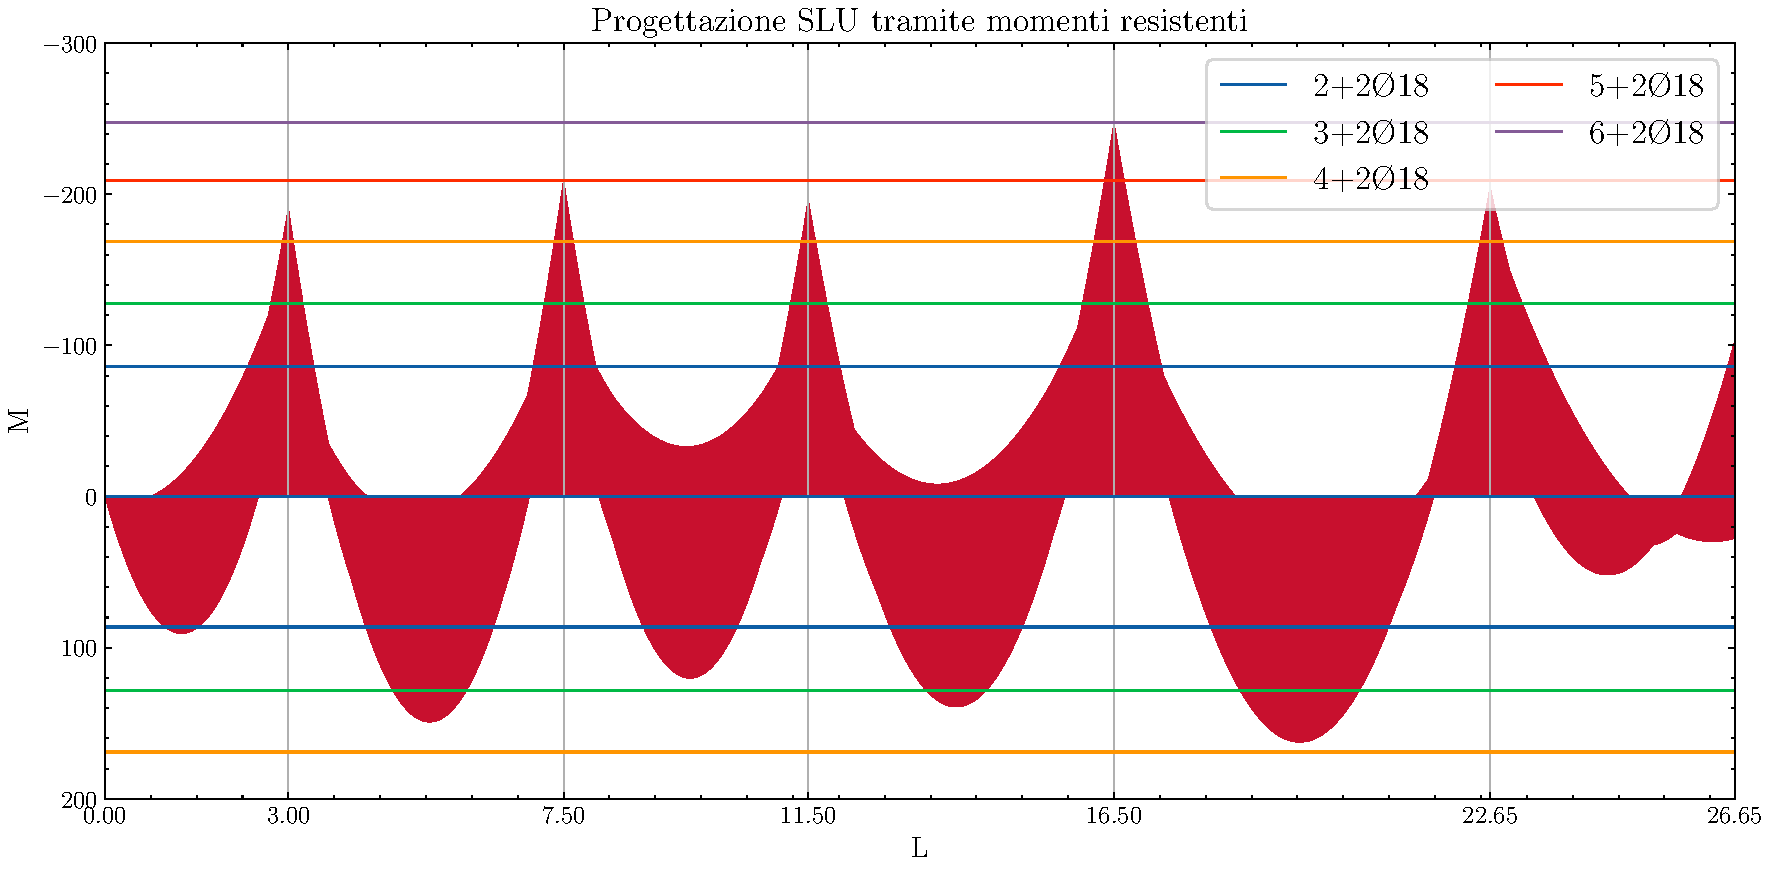
\includegraphics[width=\textwidth]{IMG/ULS_M_progettazioneTramiteMomentiResistenti.pdf}
  \caption{Progettazione SLU tramite i momenti resistenti}
  \label{fig:ULS_M_progettazioneTramiteMomentiResistenti}
\end{figure}
Da tale progetto si sono perciò determinate i veri quantitativi di armattura da adottare in modo che venisse soddisfatta la verifica in ciascun punto.
In tabella \ref{tab:ULS_M_VerificaSezioni} sono riportati i quantitativi di armatura e i relativi momenti resistenti per le sezioni caratteristiche dell'intera trave.
%
  \begin{table}[htb]
    \centering
    \scriptsize
    \caption[Riassunto della verifica SLU a momento flettente per tutte le sezioni]{Riassunto della verifica SLU a momento flettente per tutte le sezioni. Ogni sezione si intende con caratteristiche geometriche di base e altezza uguali e con  medesimi materiali.}
    \label{tab:ULS_M_VerificaSezioni}
    \begin{tabular}{
        l
        c
        c
        S[table-format=3.3]
        l
        S[table-format=2.2]
        S[table-format=2.2]
        S[table-format=2.2]
        S[table-format=1.4]
        S[table-format=1.4]
        S[table-format=1.4]
        S[table-format=3.3]
        r
        S[table-format=2.1]}
    \toprule
    \multirow{2}{*}{Sez.}   & \multirow{2}{*}{$A_s$}    & \multirow{2}{*}{$A_s^\prime$} & {$M_{Ed}$}                    & \multirow{2}{*}{Campo}    & {$\varepsilon_c$}         & {$\varepsilon_s$}         & {$\varepsilon_s^\prime$}  & \multicolumn{1}{c}{\multirow{2}{*}{$\xi$}}    & \multicolumn{1}{c}{\multirow{2}{*}{$\psi$}}   & \multicolumn{1}{c}{\multirow{2}{*}{$\lambda$}}    & {$M_{Rd}$}                    & \multicolumn{2}{l}{$M_{Ed}<M_{Rd}$} \\
                            &                           &                               & {\si{[\kilo\newton\metre]}}   &                           &{\si{[\textperthousand]}}  &{\si{[\textperthousand]}}  &  {\si{[\textperthousand]}} &                        &                           &                               & {\si{[\kilo\newton\metre]}}   & & {\si{[\percent]}}\\
    \midrule
    A1 inv & 2Ø18 & 2Ø18 & 0.000   & 2A-1 & 1.51 & 10.00 & 0.51 & 0.1311 & 0.5648 & 0.3613 & 86.276  & \checked & 0.0 \\
    C1     & 3Ø18 & 2Ø18 & 90.595  & 2A-1 & 1.91 & 10.00 & 0.88 & 0.1607 & 0.6519 & 0.3724 & 128.015 & \checked & 70.8 \\
    A2 inv & 6Ø18 & 2Ø18 & 190.969 & 2B   & 3.40 & 10.00 & 2.23 & 0.2535 & 0.8037 & 0.4138 & 247.634 & \checked & 77.1 \\
    C2     & 4Ø18 & 2Ø18 & 149.180 & 2A-2 & 2.33 & 10.00 & 1.26 & 0.1890 & 0.7139 & 0.3856 & 168.988 & \checked & 88.3 \\
    A3 inv & 6Ø18 & 2Ø18 & 209.462 & 2B   & 3.40 & 10.00 & 2.23 & 0.2535 & 0.8037 & 0.4138 & 247.634 & \checked & 84.6 \\
    C3     & 3Ø18 & 2Ø18 & 120.204 & 2A-1 & 1.91 & 10.00 & 0.88 & 0.1607 & 0.6519 & 0.3724 & 128.015 & \checked & 93.9 \\
    A4 inv & 6Ø18 & 2Ø18 & 196.601 & 2B   & 3.40 & 10.00 & 2.23 & 0.2535 & 0.8037 & 0.4138 & 247.634 & \checked & 79.4 \\
    C4     & 4Ø18 & 2Ø18 & 139.165 & 2A-2 & 2.33 & 10.00 & 1.26 & 0.1890 & 0.7139 & 0.3856 & 168.988 & \checked & 82.4 \\
    A5 inv & 6Ø18 & 2Ø18 & 247.450 & 2B   & 3.40 & 10.00 & 2.23 & 0.2535 & 0.8037 & 0.4138 & 247.634 & \checked & 99.9 \\
    C5     & 4Ø18 & 2Ø18 & 162.530 & 2A-2 & 2.33 & 10.00 & 1.26 & 0.1890 & 0.7139 & 0.3856 & 168.988 & \checked & 96.2 \\
    A6 inv & 6Ø18 & 2Ø18 & 204.824 & 2B   & 3.40 & 10.00 & 2.23 & 0.2535 & 0.8037 & 0.4138 & 247.634 & \checked & 82.7 \\
    C6     & 2Ø18 & 2Ø18 & 51.884  & 2A-1 & 1.51 & 10.00 & 0.51 & 0.1311 & 0.5648 & 0.3613 & 86.276  & \checked & 60.1 \\
    A7 inv & 3Ø18 & 2Ø18 & 103.039 & 2A-1 & 1.91 & 10.00 & 0.88 & 0.1607 & 0.6519 & 0.3724 & 128.015 & \checked & 80.5 \\
    \midrule
    A1     & 2Ø18 & 2Ø18 & 0.000   & 2A-1 & 1.51 & 10.00 & 0.51 & 0.1311 & 0.5648 & 0.3613 & 86.276  & \checked & 0.0 \\
    C1 inv & 2Ø18 & 3Ø18 & 15.137  & 2A-1 & 1.42 & 10.00 & 0.42 & 0.1241 & 0.5410 & 0.3591 & 86.200  & \checked & 17.6 \\
    A2     & 2Ø18 & 6Ø18 & 0.000   & 2A-1 & 1.26 & 10.00 & 0.28 & 0.1119 & 0.4978 & 0.3555 & 86.004  & \checked & 0.0 \\
    C2 inv & 2Ø18 & 4Ø18 & 0.000   & 2A-1 & 1.35 & 10.00 & 0.36 & 0.1189 & 0.5230 & 0.3575 & 86.126  & \checked & 0.0 \\
    A3     & 2Ø18 & 6Ø18 & 0.000   & 2A-1 & 1.26 & 10.00 & 0.28 & 0.1119 & 0.4978 & 0.3555 & 86.004  & \checked & 0.0 \\
    C3 inv & 2Ø18 & 3Ø18 & 33.154  & 2A-1 & 1.42 & 10.00 & 0.42 & 0.1241 & 0.5410 & 0.3591 & 86.200  & \checked & 38.5 \\
    A4     & 2Ø18 & 6Ø18 & 0.000   & 2A-1 & 1.26 & 10.00 & 0.28 & 0.1119 & 0.4978 & 0.3555 & 86.004  & \checked & 0.0 \\
    C4 inv & 2Ø18 & 4Ø18 & 10.062  & 2A-1 & 1.35 & 10.00 & 0.36 & 0.1189 & 0.5230 & 0.3575 & 86.126  & \checked & 11.7 \\
    A5     & 2Ø18 & 6Ø18 & 0.000   & 2A-1 & 1.26 & 10.00 & 0.28 & 0.1119 & 0.4978 & 0.3555 & 86.004  & \checked & 0.0 \\
    C5 inv & 2Ø18 & 4Ø18 & 0.000   & 2A-1 & 1.35 & 10.00 & 0.36 & 0.1189 & 0.5230 & 0.3575 & 86.126  & \checked & 0.0 \\
    A6     & 2Ø18 & 6Ø18 & 0.000   & 2A-1 & 1.26 & 10.00 & 0.28 & 0.1119 & 0.4978 & 0.3555 & 86.004  & \checked & 0.0 \\
    C6 inv & 2Ø18 & 2Ø18 & 18.039  & 2A-1 & 1.51 & 10.00 & 0.51 & 0.1311 & 0.5648 & 0.3613 & 86.276  & \checked & 20.9 \\
    A7     & 2Ø18 & 3Ø18 & 27.682  & 2A-1 & 1.42 & 10.00 & 0.42 & 0.1241 & 0.5410 & 0.3591 & 86.200  & \checked & 32.1 \\
    \bottomrule
    \end{tabular}
    \end{table}

\section{Traslazione del diagramma dei momenti sollecitanti e diagramma del momento resistente}
Prima di poter rappresentare il vero diagramma dei momenti reistenti è necessario traslare il diagramma dei momenti sollecitanti per far fronte al contributo sollecitante dovuto alla trazione che le armature tese aggiungono.

Tale valore di traslazione è possibile calcolarlo mediante la formula \normaref{4.1.30} delle \norma{NTC18} e vale:
\begin{equation}
    a_1 = \frac{0.9 \, d \, \cot\vartheta}{2} \; \text{nel verso meno favorevole} \quad.
\end{equation}
Essendo $\vartheta$ limitato da normativa, si sceglie il meno favorevole corrispondente a $\cot\vartheta = 2.5$. 
Pertanto il quantitativo da traslare è pari a 
\[
    a_1 = \frac{0.9 \, \SI{460}{\milli\metre} \, 2.5}{2} = \SI{0.5175}{\metre} \quad
\]
e la precedente raffigurazione di figura \ref{fig:ULS_M_progettazioneTramiteMomentiResistenti} diviene ora quella della figura \ref{fig:ULS_M_progettazioneTramiteMomentiResistenti_trasposto}.
\begin{figure}[htb]
  \centering
  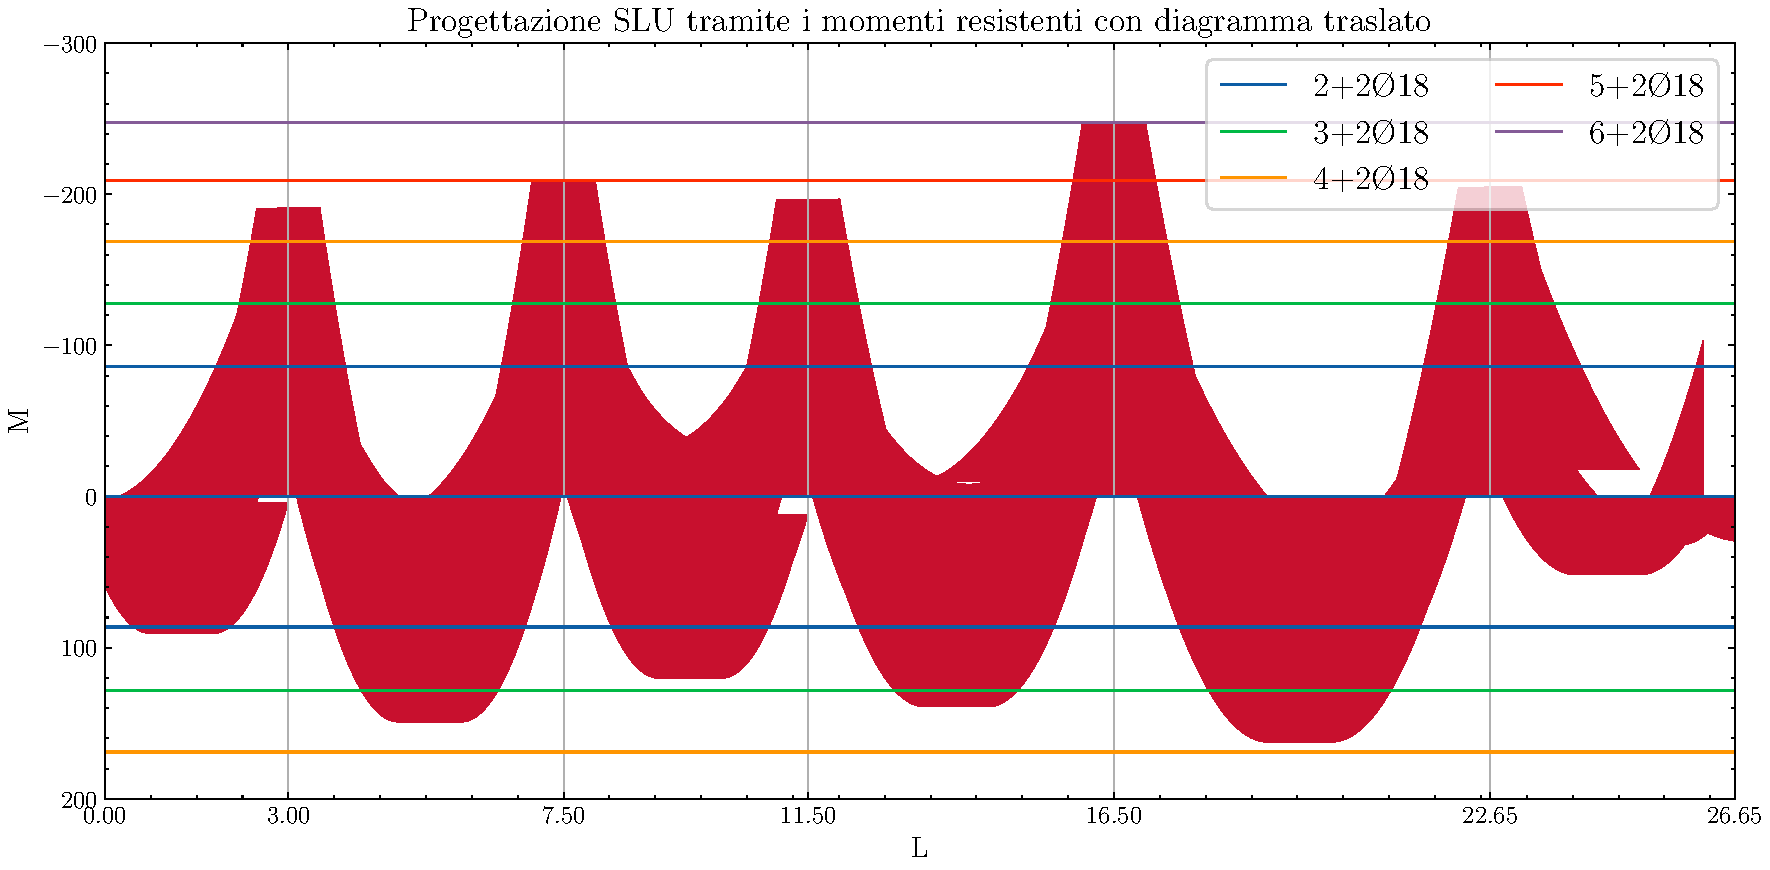
\includegraphics[width=\textwidth]{IMG/ULS_M_progettazioneTramiteMomentiResistenti_traslato.pdf}
  \caption{Progettazione SLU tramite i momenti resistenti con diagramma traslato}
  \label{fig:ULS_M_progettazioneTramiteMomentiResistenti_traslato}
\end{figure}

\section{Lunghezza di ancoraggio e disposizione finale delle armature}
Per ottenere la disposizione finale della armature è necessario calcolare il quantitativo minimo di cui la barre devono sovrapporsi.
Tale lunghezza di ancoraggio è possibile calcolarla facendo riferimento all'\norma{EC2} al \normaref{\S 8.4} e deve essere sosfatto $l_b l_{b,req}> $

\[
\begin{split}
f_{bd} 
&= 2.25 \cdot \eta_{1} \cdot \eta_{2} \cdot f_{ctd}  
= 2.25 \cdot 1 \cdot 1 \cdot \SI{1.197}{\mega\pascal} 
= \SI{2.693}{\mega\pascal}  
\\
l_{b,req} 
&= d_{barre} \frac{ \sigma_{d} }{ 4 \cdot f_{bd} }  
= \SI{18}{\milli\metre}  \frac{ \SI{391.304}{\mega\pascal} }{ 4 \cdot \SI{2.693}{\mega\pascal} } 
= \SI{653.808}{\milli\metre}  
\\
l_{b,min} 
&= 
\max { \left( 0.3 \, l_{b,req} ,\  10 \, d_{barre} ,\  100 \right) }  
= \max { \left( 0.3 \cdot 653.808 ,\  10 \cdot 18 ,\  100 \right) } \,\si{\milli\metre}
= \SI{196.143}{\milli\metre} \; \;\textrm{trazione}
\\
l_{b,min} 
&= \max { \left( 0.6 \, l_{b,req} ,\  10 \, d_{barre} ,\  100 \right) }  
= \max { \left( 0.6 \cdot 653.808 ,\  10 \cdot 18 ,\  100 \right) } \,\si{\milli\metre}
= \SI{392.285}{\milli\metre} \; \;\textrm{compressione}
\\
l_{b} 
&= \alpha_{1} \cdot \alpha_{2} \cdot \alpha_{3} \cdot \alpha_{4} \cdot \alpha_{5} \cdot l_{b,req}  
= 1 \cdot 1 \cdot 1 \cdot 1 \cdot 1 \cdot \SI{653.808}{\milli\metre} 
= \SI{653.808}{\milli\metre} > l_{b,min} \quad \checked
\end{split}
\]
in cui tutti i coefficienti $\alpha$ valgono $1$ in quanto le barre sono dritte, il riprimento delle barre e il confinamento è adeguato, le barre non sono saldate e non c'è pressione trasversale.
I coefficienti $\eta$ corrispondono a barre con buona aderenza e con diametro minore al Ø18.
Non avendo problemi di dimensione agli appoggi (essendo la trave ad altezza fuori spessore) la sollecitazione $\sigma_{d}$ delle barre è stata presa quella massima possibile, senza effettuare calcoli più raffinati.

La lunghezza di ancoraggio è perciò pari a circa \SI{66}{\centi\metre}.
In appoggio tale lunghezza è considerata fino a metà pilastro, per poi svoltare verticalmente all'interno di esso.

Una disposizione schematica delle armature è visibile in figura \ref{fig:ULS_M_ULS_M_DisposioneArmature}: si è cercato di semplificare il più possibile la loro disposizione ed eliminare le zone in cui ci sarebbe stata una barra molto corta. 
Tra il primo e il secondo appoggio, nella parte di momento positivo, ne è un esempio.
\begin{figure}[htb]
  \centering
  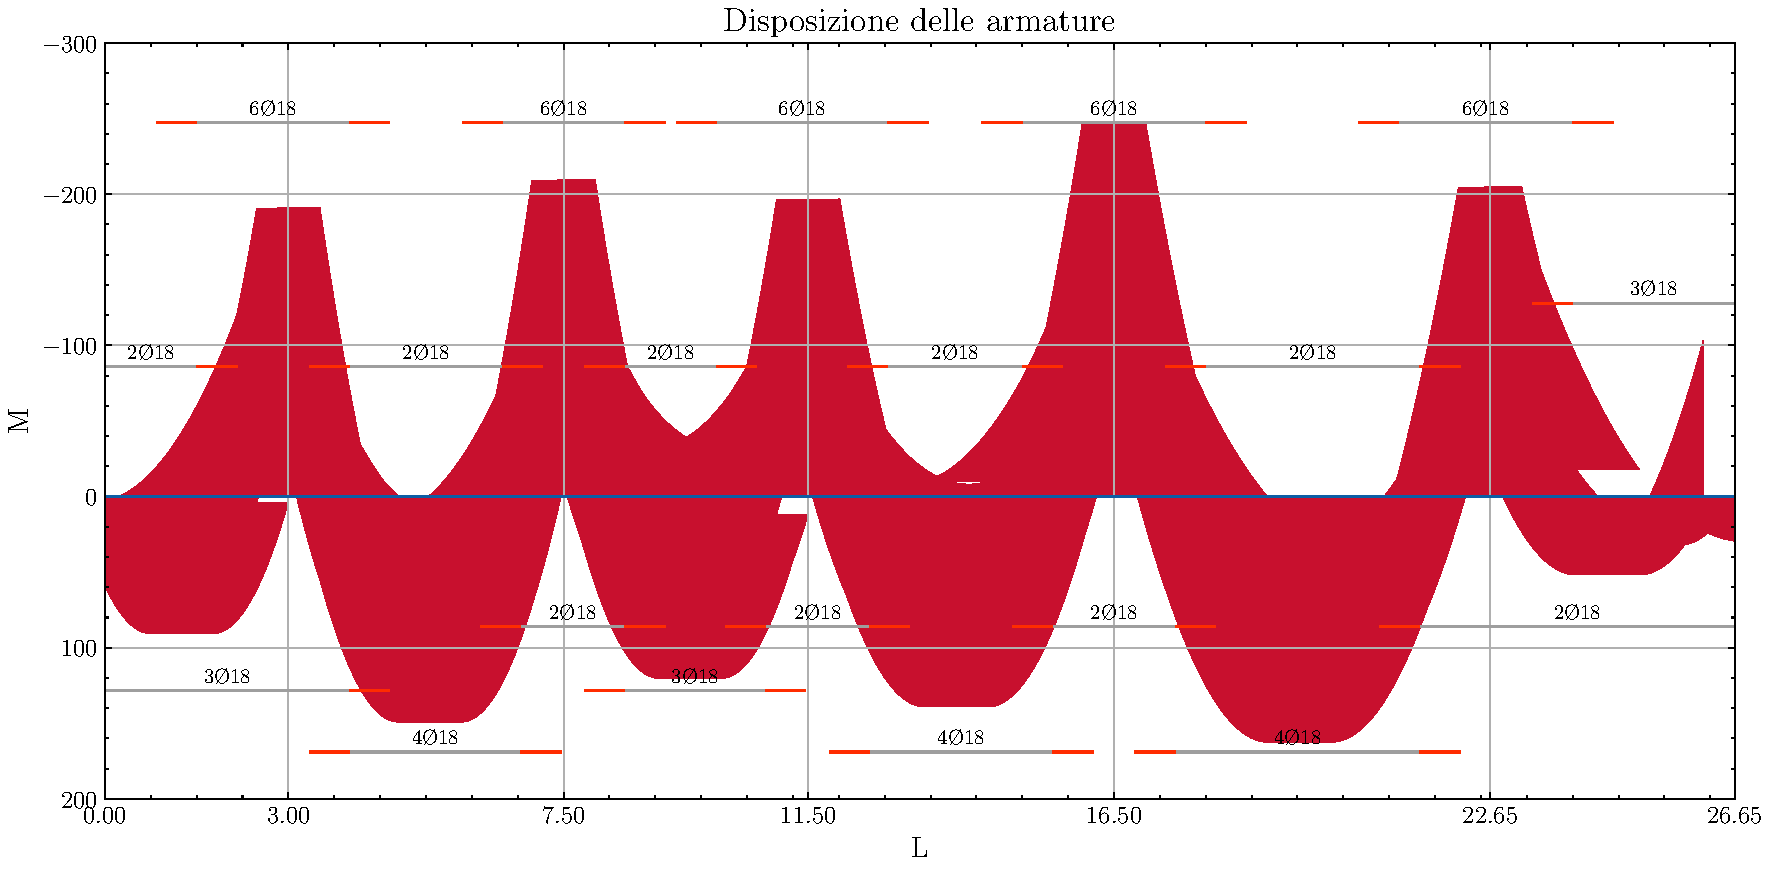
\includegraphics[width=\textwidth]{IMG/ULS_M_DisposioneArmature.pdf}
  \caption{Disposizione schematica della armatura con raffigurazione della lunghezza di ancoraggio}
  \label{fig:ULS_M_ULS_M_DisposioneArmature}
\end{figure}